\lab{Inverse Problems}{Inverse Problems}
\label{lab:inverse_problems}
\labdependencies{HeatFlow}

An important concept in mathematics is the idea of a well posed problem.
The concept initially came from Jacques Hadamard.
A mathematical problem is \textit{well posed} if 
\begin{enumerate}
	\item a solution exists, 
	\item that solution is unique, and 
	\item the solution is continuously dependent on the data in the problem.
\label{inverse_problems:continuous_dependence}
\end{enumerate}
A problem that is not well posed is \textit{ill posed}.
Notice that a problem may be well posed, and yet still possess the property that small changes in the data result in larger changes in the solution; in this case the problem is said to be \text{ill conditioned}, and has a large \text{condition number}.

Note that for a physical phenomena, a well posed mathematical model would seem to be a necessary requirement!
However, there are important examples of mathematical problems that are ill posed.
For example, consider the process of differentiation.
Given a function $u$ together with its derivative $u'$, let $\tilde{u}(t) = u(t) +  \epsilon \sin(\epsilon^{-2}t)$ for some small $\epsilon > 0$.
Then note that 
\begin{align*}
	\|u-\tilde{u}\|_{\infty} &= \epsilon,
\end{align*}
while
\begin{align*}
	\|u'-\tilde{u}'\|_{\infty} &= \epsilon^{-1}.
\end{align*}
Since a small change in the data leads to an arbitrarily large change in the output, differentiation is an ill posed problem.
And we haven't even mentioned numerically approximating a derivative!

For an example of an ill posed problem from PDEs, consider the backwards heat equation with zero Dirichlet conditions: 
\begin{align}
\begin{split}
	&{} u_t = -u_{xx}, \quad (x,t) \in (0,L)\times (0,\infty),\\
	&{} u(0,t) = u(L,t) = 0, \quad t \in (0,\infty),\\
	&{} u(x,0) = f(x), \quad x \in (0,L).
\end{split}
\end{align}
For the initial data $f(x)=0$, the unique\footnote{See \textit{Partial Differential Equations} by Lawrence C. Evans, chapter 2.3, for a proof of uniqueness.} solution is $u(x,t) = 0.$ 
Given the initial data $f(x) = \frac{1}{n}\sin ( \frac{n \pi x}{L})$, one can check that there is a unique solution $u(x,t) = \frac{1}{n}\sin ( \frac{n \pi x}{L})\exp ( (\frac{n \pi }{L})^2 t)$. 
Thus, on a finite interval $[0,T]$, as $n \to \infty$ we see that a small difference in the initial data results in an arbitrarily large difference in the solution.

\section*{Inverse Problems}
As implied by the name, inverse problems come in pairs.
For example, differentiation and integration are inverse problems.
The easier problem (in this case integration) is often called the direct problem.
Historically, the direct problem is usually studied first.

Given a physical system, together with initial data (the ``cause''), the direct problem will usually predict the future state of the physical system (the ``effect''); see Figure \ref{fig:cause_and_effect}.
Inverse problems often turn this on its head---given the current state of a physical system at time $T$, what was the physical state at time $t = 0$?  

Alternatively, suppose we measure the current state of the system, and we then measure the state at some future time.
An important inverse problem is to determine an appropriate mathematical model that can describe the evolution of the system.

\begin{figure}
\centering
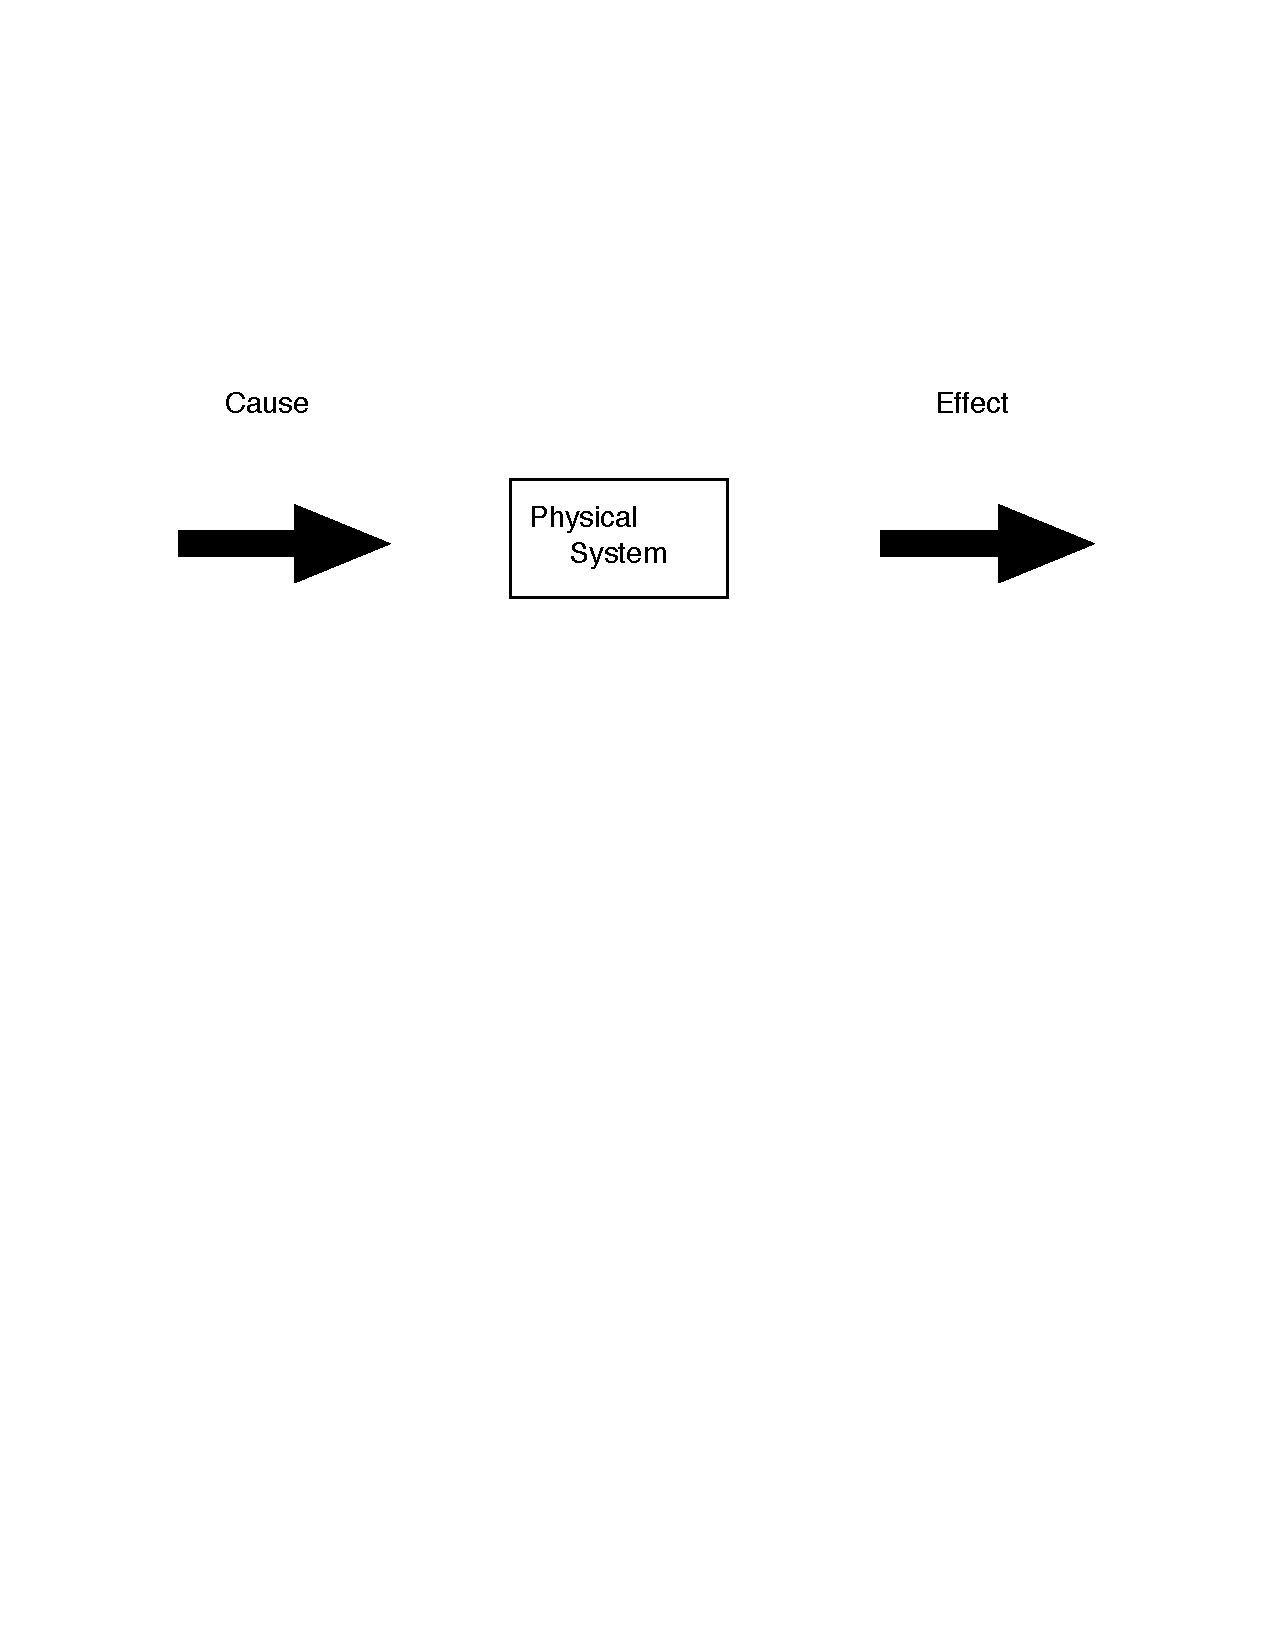
\includegraphics[width=\textwidth]{figures/cause_and_effect.pdf}
\caption{Cause and effect within a given physical system.}
\label{fig:cause_and_effect}
\end{figure}

\section*{Another look at heat flow through a rod}
Consider the following ordinary differential equation, together with natural boundary conditions at the ends of the interval\footnote{This example of an ill-posed problem is given in \textit{Inverse Problems in the Mathematical Sciences} by Charles W Groetsch.}:
\begin{align}
\begin{cases}
	-(au')' = f, & x \in (0,1),\\
	a(0)u'(0) = c_0, & a(1)u'(1) = c_1.
\end{cases} \label{inverse_problems:heat_flow}
\end{align}
This BVP can, for example, be used to describe the flow of heat through a rod.
The boundary conditions would correspond to specifying the heat flux through the ends of the rod.
The function $f(x)$ would then represent external heat sources along the rod, and $a(x)$ the thermal conductivity of the rod at each point. 

Typically, the thermal conductivity $a(x)$ would be specified, along with any heat sources $f(x)$, and the (direct) problem is to solve for the steady-state heat distribution $u(x)$.
Here we shake things up a bit: suppose the heat sources $f$ are given, and we can measure the heat distribution $u(x)$.
Can we find the thermal conductivity of the rod?
This is an example of a \textit{parameter estimation problem}.

Let us consider a numerical method for solving \eqref{inverse_problems:heat_flow} for the thermal conductivity $a(x)$.
Subdivide $[0,1]$ into $N$ equal subintervals, and let $x_j = jh$, $j = 0, \ldots,N$, where $h = 1/N$.
Let $\phi_j(x)$ be the tent functions (used earlier in the finite element lab), given by 
\begin{align*}
	\phi_j(x) = \begin{cases}
(x - x_{j-1})/h  &  x \in [x_{j-1},x_j],\\
 (x_{j+1} - x)/h  &  x \in [x_{j},x_{j+1}],\\
0 & \text{ otherwise.}
\end{cases}
\end{align*}
We look for an approximation $a^h(x)$ that is a linear combination of tent functions. This will be of the form 
\begin{align}
	a^h &= \sum_{j=0}^N \alpha_j \phi_j, \quad \alpha_j=a(x_j).
\label{inverse_problems:approximate}
\end{align}
The $h$ in this equation indicates that each of the tent functions in the linear combination rely on $h= 1/N$, and that a different $h$ or $N$ will result in different tent functions, so $a^h$ will be different. 
The second half of \eqref{inverse_problems:approximate} says that a good choice of $a^h$ is found by taking $\alpha_j = a(x_j)$.
Integrating \eqref{inverse_problems:heat_flow} from $0$ to $x$, we obtain
\begin{align}
\begin{split}
&{} \int_0^x -(au')'\, ds = \int_0^x f(s)\, ds,\\
&{} -[a(x)u'(x) - c_0] = \int_0^x f(s)\, ds,\\
&{} u'(x) = \frac{c_0 - \int_0^x f(s)\, ds}{a(x)}.
\end{split}
\end{align}
Thus for each $x_j$
\begin{align*}
	u'(x_j) &= \frac{c_0 - \int_0^{x_j} f(s)\, ds}{a(x_j)},\\
	&= \frac{c_0 - \int_0^{x_j} f(s)\, ds}{\alpha_j}.
\end{align*}
The coefficients $\alpha_j$ in \eqref{inverse_problems:approximate} can now be approximated as $\alpha^*_j$ by minimizing 
\begin{align}
	\alpha^*_j = \arg\min_{\alpha_j}\left\{\left( \frac{c_0 - \int_0^{x_j} f(s)\, ds}{\alpha_j} - u'(x_j)  \right)^2\right\}.
\label{eqn:inverse:min_alpha}
\end{align}


\begin{figure}[H]
\centering
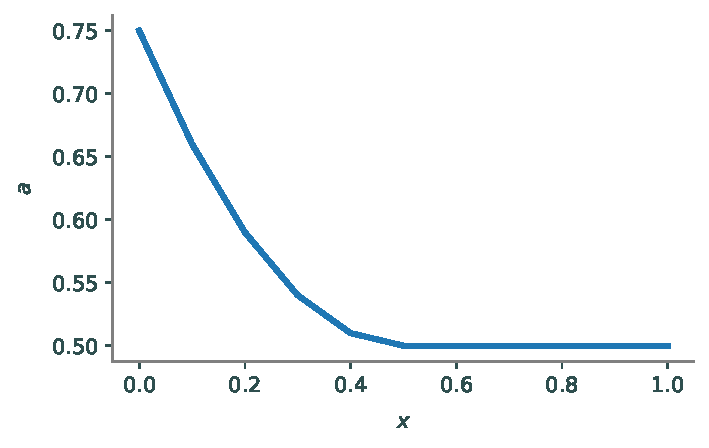
\includegraphics[width=\textwidth]{figures/density_a.pdf}
\caption{The solution $a(x)$ to Problem \ref{prob:inverse}}
\label{fig:inverse_problems:num1}
\end{figure}

\begin{problem}
Use \eqref{eqn:inverse:min_alpha} to solve \eqref{inverse_problems:heat_flow} for $a(x)$ using the following conditions:

\noindent $c_0 = 3/8,$ $c_1 = 5/4$, $u(x) = x^2 + x/2 + 5/16$, $x_j=0.1j$ for $j=0,1,\dots,10$, and 
\begin{align*}
	f &= \begin{cases}
		-6x^2 + 3x - 1 & x \leq 1/2,\\
		-1 & 1/2 < x \leq 1,
	\end{cases}
\end{align*}
Produce the plot shown in Figure \ref{fig:inverse_problems:num1}.

Hint: use the \li{minimize} function in \li{scipy.optimize} and some initial guess to find the $\alpha_j$.
 Alternatively, notice that \eqref{eqn:inverse:min_alpha} is simple enough that it can be solved explicitly for $\alpha_j$.
\label{prob:inverse}
\end{problem}

\begin{problem}
	Find the thermal conductivity function $a(x)$ satisfying 
	\begin{align}
	\begin{cases}
		-(au')' = -1, & x \in (0,1),\\
		a(0)u'(0) = 1, & a(1)u'(1) = 2.
	\end{cases} \label{inverse_problems:ill_posed}
	\end{align}
	where $u(x) = x + 1 + \epsilon \sin(\epsilon^{-2}x)$. 
Using several values of $\epsilon  > 0.66049142$, plot the corresponding thermal conductivity $a(x)$ for $x$ in \li{np.linspace(0,1,11)} to demonstrate that the problem is ill-posed, as in Figure \ref{fig:inverse_problems:exercise1}.
Be sure to add a legend to your plot.
\end{problem}

\begin{figure}[H]
\centering
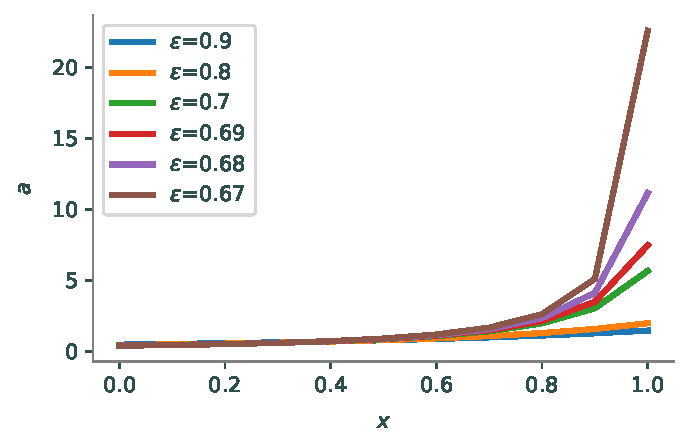
\includegraphics[width=\textwidth]{figures/ill_posed_density_a.pdf}
\caption{The thermal conductivity function $a(x)$ satisfying \eqref{inverse_problems:ill_posed} for $\epsilon = 0.8$.}
\label{fig:inverse_problems:exercise1}
\end{figure}

\section*{Time-Dependent Inverse Problems}
We can also expand our use of inverse problems from time-independent PDEs to time-dependent variables. In this section of the lab, we will do it with the nonlinear time-dependent diffusion equation. We will also introduce noise to the measurements, making this much more realistic.

\subsection*{Time-Dependent Heat Diffusion Update}
The nonlinear time-dependent diffusion equation is
\begin{align}
\begin{split}
\frac{\partial}{\partial t}u(x,t) &= \frac{\partial}{\partial x}\left(\nu(x)\frac{\partial u(x,t)}{\partial x}\right)\\
&= \left(\frac{\partial\nu(x)}{\partial x}\right)\left(\frac{\partial u(x,t)}{\partial x}\right)+\nu(x)\left(\frac{\partial^2 u(x,t)}{\partial x^2}\right).
\end{split}
\label{eqn:inverse:nonlinear_diffusion}
\end{align}

Note that this form of the diffusion equation is slightly more general than the one in the heat diffusion lab, since the diffusion coefficient $\nu$ is not a constant. 

If our spatial grid is indexed by $j\in\{0, \ldots, J-1\}$ with step $h$, and our time grid is indexed by $m\in\{0, \ldots, M-1\}$ with step $k$, then the time derivative can be approximated as
\begin{equation*}
	u_t(x_j, t_m) = \frac{u(x_j, t_m + k) - u(x_j, t_m)}{k} + \mathcal{O}(k).
\end{equation*}
and the second-order centered difference approximation for the second spatial derivative is
\begin{equation*}
	u_{xx}(x_j,t_m) = \frac{u(x_j + h,t_m )-2 u(x_j,t_m)+ u(x_j - h,t_m)}{h^2} + \mathcal{O}(h^2).
\end{equation*}
The second-order centered difference approximations for the first spatial derivatives (of $u$ and $\nu$) are
\begin{align*}
	u_x(x_j, t_m) &= \frac{u(x_j + h, t_m) - u(x_j - h, t_m)}{2h} + \mathcal{O}(h^2)\\
	\nu_x(x_j) &= \frac{\nu(x_j + h) - \nu(x_j - h)}{2h} + \mathcal{O}(h^2).
\end{align*}
Letting $\vec \nu$ be a vector of $\nu_j = \nu(x_j)$ evaluated at each grid point in space, the update iteration scheme then becomes

\begin{equation}
U_{j}^{m+1}(\vec \nu) = U_{j}^{m} + \frac{ k}{h^2} \left[ \nu_j(U_{j+1}^m - 2U_{j}^{m} + U_{j-1}^{m} ) + \left(\frac{(\nu_{j+1}-\nu_{j-1})(U^m_{j+1}-U^m_{j-1})}{4}\right)\right].
\label{eqn:inverse:diffusion_update}
\end{equation}
where we omit (or suppress) the dependence of $U_j^m$, $U_{j+1}^m$, and $U_{j-1}^m$ on $\vec \nu$ for brevity.
Note that this update equation is the same as the one in the Heat Diffusion Lab, but with an added last term.

\subsection*{Inverse Problems with Noise}

We want to find the heat diffusion coefficient $\vec \nu$ that minimizes the difference between the measured heat $\hat U$ and our approximation $U(\vec \nu)$ which we compute using \eqref{eqn:inverse:diffusion_update}. That is, we want to find $\vec \nu$ such that the sum of squared errors

\begin{align}
\text{SSE} = \sum_{j=0}^{J-1} \sum_{m=0}^{M-1} [U_j^m(\vec \nu) - \hat U_j^m]^2
\label{eqn:inverse:sse}
\end{align}

\noindent is minimized.
Note that since $\hat U$ is a measurement of a true heat distribution $u^*(x,t)$, it is subject to noise.
Also note that this is a least-squares problem (like Problem \ref{prob:inverse}), but the solution is not trivial since each $\nu_j$ is constant in time, but multiple noisy measurements are taken at the same point $x_j$ at different times $t_m$.

To solve this problem, we will choose a guess for our initial heat diffusion coefficient, solve for the heat flow using our guess, and then using a minimization method (such as BFGS), we will update our vector of parameters, $\vec \nu$. Here is some code to help get you started:

\begin{lstlisting}
# This is an MxJ matrix of measured, noisy data.
U_hat = np.load('measured_heat.npy')
M, J = U_hat.shape

def sse(nu, U_hat):

    # Initialize U with the the first row (time) of `U_hat`, then loop
    # forward in time using `nu` and equation (8).

    return # Result of equation (9)

# This is a good guess. There are others that will work fine too.
guess = np.full(J, 2)

sol = minimize(sse, guess, args=U_hat, method='BFGS')
nu = sol.x
\end{lstlisting}

\begin{problem}
The file \li{measured_heat.npy} contains measurements over time ($t \in [0, 2]$) of the temperature along an insulated rod with a varying diffusion coefficient $\nu(x)$.
The first row corresponds to the iniital state of the heat distribution in the rod.
Use equation \eqref{eqn:inverse:diffusion_update} and the code above to find an estimate $\vec \nu$ of $\nu(x)$ that minimizes the sum of squared errors \eqref{eqn:inverse:sse}.
For $x \in [-10, 10]$, plot $\vec \nu$ along with the true $\nu(x)$, which is given by
\begin{align*}
\nu(x) = \frac{5}{1+e^{-x}}+\frac{1}{2}.
\end{align*}
Compare with Figure \ref{fig:inverse_problems:find_nu}.
Be sure to add a legend to your plot.
Notice that the model does worse at the endpoints.
This is partially because the endpoints in the PDE are fixed at zero with Dirichlet conditions, so the value of $\nu$ at the endpoints has little little effect on the evolution of the PDE.

Hint: Use array broadcasting when possible. Note that the array in \li{measured_heat.npy} is $21 \times 11$, so $M = 21$ and $J = 11$.
\label{inverse_problems:varying_nu}
\end{problem}

\begin{figure}[H]
\centering
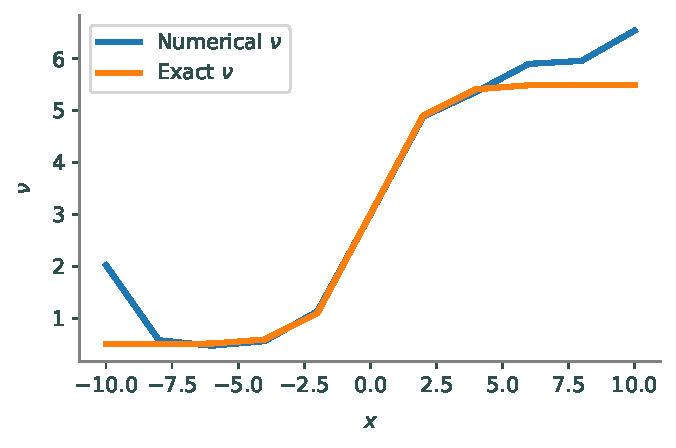
\includegraphics[width=\textwidth]{figures/spatially_dependent_nu.pdf}
\caption{Solution to Problem \ref{inverse_problems:varying_nu}}
\label{fig:inverse_problems:find_nu}
\end{figure}
